\documentclass[twocolumn,english]{article}
\usepackage[latin9]{inputenc}
\usepackage[landscape]{geometry}
\geometry{verbose,tmargin=0.5in,bmargin=0.75in,lmargin=0.5in,rmargin=0.5in}
\setlength{\parskip}{0bp}
\setlength{\parindent}{0pt}
\usepackage{float}
\usepackage{booktabs}
\usepackage{amsmath}
\usepackage{graphicx}
\PassOptionsToPackage{normalem}{ulem}
\usepackage{ulem}

\makeatletter

\providecommand{\tabularnewline}{\\}




\usepackage{array}
\usepackage{multirow}
\usepackage{amsbsy}




\providecommand{\tabularnewline}{\\}

\setlength{\columnsep}{0.25in}
\usepackage{xcolor}
\usepackage{textcomp}
\usepackage{listings}
\lstset{
  tabsize=2,
  basicstyle=\small\ttfamily,
}



\usepackage{babel}
\usepackage{listings}
\renewcommand{\lstlistingname}{Listing}

\makeatother

\usepackage{babel}
\usepackage{listings}
\renewcommand{\lstlistingname}{Listing}

\begin{document}

\title{Reference Sheet for C212 Networks and Communications}

\date{Autumn 2017}
\maketitle

\section{The Internet}

\begin{figure}[H]
\centering{}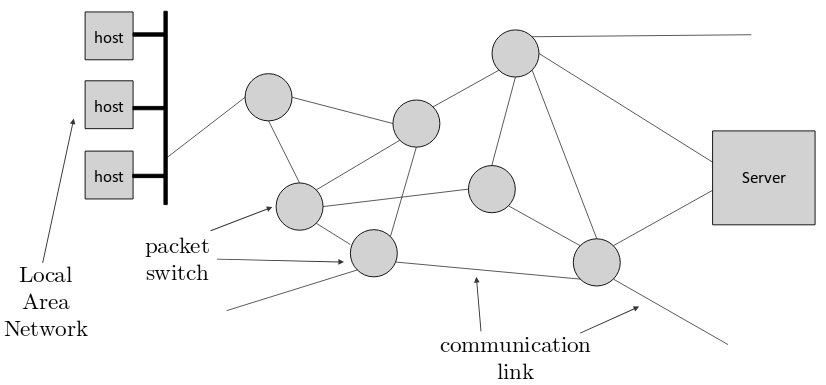
\includegraphics[width=0.75\linewidth]{img/internet}
\end{figure}
\begin{itemize}
\item \emph{Packet switch}: link-layer switch or router.
\item \emph{Communication link}: connection between packet switches and/or
end systems.
\begin{itemize}
\item Fibre optic cable, twisted pair copper wire, coaxial cable, wireless
local area links, etc.
\end{itemize}
\item \emph{Route} (\emph{path}): sequence of switches a packet goes through.
\item \emph{Protocol}: control the sending and receiving of information
between end systems/packet switches
\end{itemize}

\paragraph{Packet Switching vs Circuit Switching}

Packet-switched networks (e.g. the Internet):
\begin{enumerate}
\item Information transmitted in \emph{packets}: formatted unit of data.
\item Switches/routers operate on individual packets.
\item Switches/routers receive packets and \emph{forward} them - forwarding
decision taken on the basis of information within the packet.
\end{enumerate}
Circuit-switched networks (e.g. the telephone network):
\begin{enumerate}
\item Has a setup phase: network reserves all resources for the connection
(links, buffers, switches, etc.).
\item Links are dedicated for the entire duration of the connection.
\item Connection is destroyed and resources are freed.
\end{enumerate}
Comparing packet and circuit switching:
\begin{itemize}
\item Packet switching is \emph{connectionless}, circuit switching is \emph{connection-oriented}.
\end{itemize}
\begin{table}[H]
\centering{}%
\begin{tabular}{ccc}
\toprule 
 & \textbf{\footnotesize{}Packet Switching} & \textbf{\footnotesize{}Circuit Switching}\tabularnewline
\midrule
\emph{\footnotesize{}Setup cost} & {\footnotesize{}None} & {\footnotesize{}Expensive}\tabularnewline
\emph{\footnotesize{}Processing cost} & {\footnotesize{}For each forward} & {\footnotesize{}Little / none}\tabularnewline
\emph{\footnotesize{}Space overhead} & {\footnotesize{}For each packet} & {\footnotesize{}Little / none}\tabularnewline
\emph{\footnotesize{}Quality of Service} & {\footnotesize{}Difficult to guarantee} & {\footnotesize{}Easily guaranteed}\tabularnewline
\emph{\footnotesize{}Utilisation of links} & {\footnotesize{}Shares links - efficient} & {\footnotesize{}Limited sharing - inefficient}\tabularnewline
\bottomrule
\end{tabular}
\end{table}

\paragraph{Communication Protocols}

An agreement on how communication is to proceed.
\begin{itemize}
\item Must be an \emph{executable specification} which is \emph{unambiguous}
and \emph{complete}.
\item Needs to be able to solve \emph{addressing}, \emph{error control},
\emph{flow control}, \emph{multiplexing}/\emph{demultiplexing} and
\emph{routing}.
\end{itemize}
\begin{enumerate}
\item \emph{Handshake}: establish identities and/or contact.
\item \emph{Conversation}: exchange information.
\item \emph{Closing}: terminate conversation.
\end{enumerate}
\emph{Protocol Layering}:

\begin{figure}[H]
\centering{}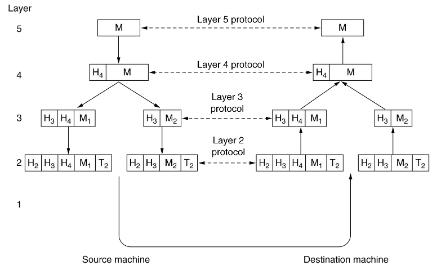
\includegraphics[width=0.5\linewidth]{img/protocol-layering}
\end{figure}
\begin{itemize}
\item \emph{Service}: set of primitives that layer provides to the layer
above.
\item \emph{Protocol}: set of rules that prescribe layout and meaning of
packets, and how the should be sent.
\item Layer $k$ puts its packet as data into a layer $k-1$ packet - which
may add a header and/or trailer.
\item \emph{Fragmentation} may be required: layer $k$ data may have to
be split accross several layer $k-1$ packets.
\end{itemize}
\emph{Internet Protocol Stack}:
\begin{enumerate}
\item \emph{Application}: defines application functionality and message
formats. E.g. Web (HTTP/HTTPS), E-mail (SMTP), BitTorrent, etc.
\item \emph{Transport}: offers connection-oriented and connectionless services.
Usually:
\begin{enumerate}
\item provides interface through \emph{sockets}, 
\item allows setting up connection, and delivering data reliably and in
the order it was sent,
\item ensures fast senders don't overwhelm slow receivers (\emph{flow control}),
\item supports \emph{secure connections}.
\end{enumerate}
\item \emph{Network (Internet)}: describes how \emph{routing} and \emph{congestion}
is solved.
\item \emph{Data Link}: allows computers to share common channel and detects
transmission errors (e.g. parity bit, checksum). E.g. Ethernet.
\item \emph{Physical}: describes transmissions of raw bits.
\end{enumerate}

\paragraph{Data Transfer}
\begin{itemize}
\item \emph{Bandwidth}: amount of information that can enter (or leave)
a connection per time unit.
\item \emph{Throughput}: actual amount of information that enters (or leaves)
connection per time unit.
\item \emph{Latency}: time it takes for one bit to go through the connection.
\item \emph{Transfer time}, $\Delta$ $=$ propagation delay (latency),
$d$ $+$ transmission delay (packet size, $L$ $/$ throughput, $R$).
\end{itemize}
With two hops, we also include \emph{router delay}, $d_{x}$, which
is made up of:
\begin{enumerate}
\item \emph{Processing delay}, $d_{\text{proc}}$: check bit errors, determine
output link (usually negligible).
\item \emph{Queuing delay}, $d_{q}$: time waiting at output link for transmission
(depends on average packet arrival rate, $a$):
\begin{enumerate}
\item $\frac{La}{R}\approx0$: small avg. queuing delay.
\item $\frac{La}{R}\rightarrow1$: large avg. queuing delay.
\item $\frac{La}{R}>1$: avg. queuing delay is infinite.
\end{enumerate}
\end{enumerate}

\section{Application Layer}

\emph{Hosts and Processes}:
\begin{itemize}
\item \emph{Host} (end system): May run multiple processes.
\item \emph{Process}: Addressed within its host by a port number.
\item \emph{Socket}: Network interface, managed by OS.
\end{itemize}
\emph{Clients and Servers}:
\begin{itemize}
\item \emph{Client}: process that initiates the communication (and establishes
connection on a connection-oriented service).
\begin{itemize}
\item Creates a socket $C$ by connecting to a server application on host
$H$ and port $P$.
\item Uses $C$ by reading and writing data into it.
\item Disconnects and destroys $C$.
\end{itemize}
\item \emph{Server}: process that waits to be contacted.
\begin{itemize}
\item Creates a socket $S$ by accepting a connection on port $P$.
\item Uses socket $S$ by reading and writing data into it.
\item Disconnects and destroys $S$.
\end{itemize}
\item \emph{Peer-to-Peer}: Processes can act as both clients and servers.
\end{itemize}

\subsection{Web (HTTP)}
\begin{itemize}
\item Uses connection-oriented transport, TCP. (port 80).
\item Consists of a sequence of requests issued by the client, and respoonses
issued by the server.
\item Stateless.
\end{itemize}

\paragraph{Requests}
\begin{enumerate}
\item Request line: \texttt{METHOD URL Protocol/Version}.
\item Header lines: \texttt{Name: Value}. 
\item Empty line.
\item Object body.
\end{enumerate}

\paragraph{Methods}
\begin{itemize}
\item \emph{GET}: retrieve object identified by URL.
\item \emph{POST}: submit data to the service.
\item \emph{OPTIONS}: request available communication options.
\item \emph{HEAD}: like GET, but without the body.
\item \emph{PUT}: store given object under given URL.
\item \emph{DELETE}: deletes given object.
\end{itemize}

\paragraph{Responses}
\begin{enumerate}
\item Status line: \texttt{Protocol/Version Code Status}.
\item Header lines: \texttt{Name: Value}.
\item Empty line.
\item Object body.
\end{enumerate}

\paragraph{Status Codes}
\begin{itemize}
\item \emph{1xx}: Informational.
\item \emph{2xx}: Successful operation.
\item \emph{3xx}: Redirection.
\item \emph{4xx}: Client error.
\item \emph{5xx}: Server error.
\end{itemize}
E.g. You can use \texttt{telnet} to make a request:

\begin{lstlisting}
telnet www.doc.ic.ac.uk 80
GET /~js4416/index.html HTTP/1.1
Host: www.doc.ic.ac.uk
\end{lstlisting}

and get a response:

\begin{lstlisting}
HTTP/1.1 200 OK
Date: ...
(Header lines) ...
Via: ...

<!DOCTYPE html>
(Page content) ...
\end{lstlisting}

\paragraph{TCP connections}
\begin{itemize}
\item HTTP/1.0 used one TCP connection per object. Now possible with \texttt{Connection: close}.
\item HTTP/1.1 introduced persistent connections - the same connection may
be used to issues multiple requests and replies.
\end{itemize}

\paragraph{Web Caching}

Improves performance and security, but adds complexity and may reduce
data `freshness'.

A client request goes to a proxy (\emph{cache}) server, which may:
\begin{enumerate}
\item Forward the request to the origin server.
\item Get the response from the origin server.
\item Store the object for some time.
\item Forward the response back to the client.
\end{enumerate}
or
\begin{enumerate}
\item Respond immediately, using a cached object.
\end{enumerate}
Implementation:
\begin{itemize}
\item Servers specify explicit expiration times using the \texttt{Expires}
header or setting \texttt{max-age} and \texttt{must-revalidate} in
the \texttt{Cache-Control} header.
\item A client or proxy can also use a \texttt{Cache-Control} header to
ensure they have a recent object. E.g. \texttt{Cache-Control: no-cache}
or \texttt{Cache-Control: max-age=60}.
\item A client or proxy can use a conditional \texttt{GET} with an \texttt{If-Modified-Since}
header.
\end{itemize}

\paragraph{Sessions}
\begin{itemize}
\item Server may use a \texttt{Set-Cookie} header, client may use \texttt{Cookie}
header.
\item Allows for sessions: users may be identified.
\end{itemize}

\paragraph{Dynamic Web Pages}
\begin{enumerate}
\item \emph{Common Gateway Interface}: identifies program and parameters
in URL, which builds and returns a webpage.
\item \emph{Scripting}: embedded scripts executed when page is processed
- may be server-side (e.g. PHP) or client side (e.g. JS).
\end{enumerate}

\subsection{Domain Name System}
\begin{itemize}
\item IPv4 (4 bytes) and IPv6 (16 bytes) addresses - easily processed by
routers.
\item Host names mapped to IP address by \emph{Domain Name System} (DNS).
\item Host names are within a hierarchical name space. There are 13 `root'
DNS servers that know where TLD servers are.
\item Each domain has an authoritative server, but caching used extensively.
\end{itemize}

\paragraph{DNS Query Types}
\begin{itemize}
\item A: maps host name to address.
\item NS: query for authoritative name server.
\item CNAME: query for a canonical (primary) name.
\item MX: query for mail exchange server.
\end{itemize}

\paragraph{DNS Protocol}
\begin{itemize}
\item Uses connectionless transport protocol, UDP (port 53).
\item Queries and replies have the same format.
\end{itemize}

\paragraph{Round Robin DNS}

Responds with a list of IP addresses , and order is changed to balance
load.

\paragraph{Tools}
\begin{itemize}
\item \texttt{host imperial.ac.uk} performs a simple DNS lookup.
\item \texttt{dig} is similar to \texttt{host -v}.
\item \texttt{nslookup imperial.ac.uk {[}ns0.ic.ac.uk{]}} queries nameservers,
you can use \texttt{-type=} for a certain query type, and can also
ask for an answer from a specific nameserver.
\end{itemize}

\paragraph{Content Distribution Networks}

Serve multiple copies at geographically distributed sites:
\begin{itemize}
\item \emph{Enter deep}: CDN servers deep into many access networks.
\item \emph{Bring home}: smaller number of large clusters in points of presence
near access networks.
\end{itemize}

\subsection{Electronic Mail}
\begin{itemize}
\item \emph{User agent} allows user to read, compose, reply to, send and
forward messages.
\item \emph{Mail servers}, accept messages for remote and local delivery
(using transport protocol), and allow user agents to access local
mailboxes (using access protocol).
\end{itemize}

\paragraph{SMTP}

Uses connection-oriented protocol, TCP.
\begin{enumerate}
\item Sets up TCP/IP connection between client and server (address can be
found from DNS).
\item Client requests server to accept its messages.
\item Server responds, so that client can send.
\end{enumerate}
Format:

\begin{lstlisting}
HELO jordanspooner.com
MAIL FROM: jordan@jordanspooner.com
RCPT TO: js4416@ic.ac.uk
DATA
From: Jordan Spooner <jordan@jordanspooner.com>
(Header lines) ...
Subject: Test Email

(Content)...
.
QUIT
\end{lstlisting}

Only supports 7-bit content - but extended by the \emph{Multipurpose
Internet Mail Extensions} (MIME) specification.

\paragraph{POP3}

Allows remote access, but assumes retrieved mail is deleted at the
server. This is solved by IMAP.

\section{Transport Layer}

\begin{table}[H]
\centering{}%
\begin{tabular}{ccc}
\toprule 
 & \textbf{\footnotesize{}TCP} & \textbf{\footnotesize{}UDP}\tabularnewline
 & \textbf{\footnotesize{}Transmission Control Protocol} & \textbf{\footnotesize{}User Datagram Protocol}\tabularnewline
\midrule
\emph{\footnotesize{}Type of service} & {\footnotesize{}Reliable connection-oriented} & {\footnotesize{}Unreliable connection-less}\tabularnewline
\emph{\footnotesize{}Data are called} & {\footnotesize{}Segments} & {\footnotesize{}Datagrams}\tabularnewline
\bottomrule
\end{tabular}
\end{table}

\paragraph{Ports}

Cross-platform process identifiers.
\begin{itemize}
\item Socket connection identified by two pairs of IP address, port number,
TCP/UDP.
\item First 1024 ports are reserved. E,g, 80 for HTTP, 443 for HTTPS, 110
for POP3, 25 for SMTP, 21 for FTP, 22 for SSH, ....
\end{itemize}
Use \texttt{netcat} to read and write across network connections.

\subsection{Transport Layer Interface}

\emph{Berkeley socket interface}:
\begin{enumerate}
\item Server and client each bind a transport-level address to a locally
created socket.
\begin{itemize}
\item \texttt{SOCKET(protocol)}: Create a new communication endpoint.
\item \texttt{BIND(socket, address)}: Attach a local address to a socket.
\end{itemize}
\item Server starts listening on this socket, waiting for connections from
clients.
\begin{itemize}
\item \texttt{LISTEN(socket, N)}: Announce willingness to accept N connections.
\end{itemize}
\item Server can accept or select connections from clients.
\begin{itemize}
\item \texttt{ACCEPT(socket)}: Block until a remote client wants to establish
connection.
\end{itemize}
\item A client connects to the socket, providing full transport-level address.
\begin{itemize}
\item \texttt{CONNECT(socket, address, port, protocol)}: Attempt to establish
a connection.
\end{itemize}
\item Client and sever communicate through send / receive operations on
their respective sockets.
\begin{itemize}
\item \texttt{SEND(socket, data)}: Send data over connection.
\item \texttt{RECEIVE(socket)}: Receive data over connection.
\end{itemize}
\item Communication ends when socket is closed.
\begin{itemize}
\item \texttt{CLOSE(socket)}: Release the connection.
\end{itemize}
\end{enumerate}
\emph{Without a connection} (e.g. UDP): no need for \texttt{LISTEN},
\texttt{ACCEPT} and \texttt{CONNECT}.

\subsection{TCP}
\begin{itemize}
\item \emph{Reliable} data transfer.
\item Uses \emph{connections}.
\item Uses \emph{congestion control}.
\item \emph{Duplex}. Both endpoints can send and receive at the same time.
\end{itemize}

\paragraph{Segmentation}

TCP data are transmitted within TCP segments.
\begin{itemize}
\item \emph{Maximum Segment Size} (MSS): maximum amount of application data
transmitted in a single segment (excluding headers).
\begin{itemize}
\item Usually related to MTU of connection, to avoid fragmentation.
\end{itemize}
\item \emph{Maximum Transmission Unit} (MTU): largest link-layer frame available
to sender.
\begin{itemize}
\item \emph{Path MTU Discovery} (PMTUD): determine largest link-layer frame
that can be sent on all links from sender host to receiver host.
\end{itemize}
\end{itemize}

\paragraph{Header Fields}
\begin{itemize}
\item \emph{Sequence number} indicates the place of the first byte carried
by the segment.
\begin{itemize}
\item When TCP connection is set up, a random \uline{I}nitial \uline{S}equence
\uline{N}umber is decided.
\end{itemize}
\item \emph{Acknowledgement number} is the first sequence number \emph{not
yet} seen by receiver.
\end{itemize}
\begin{figure}[H]
\centering{}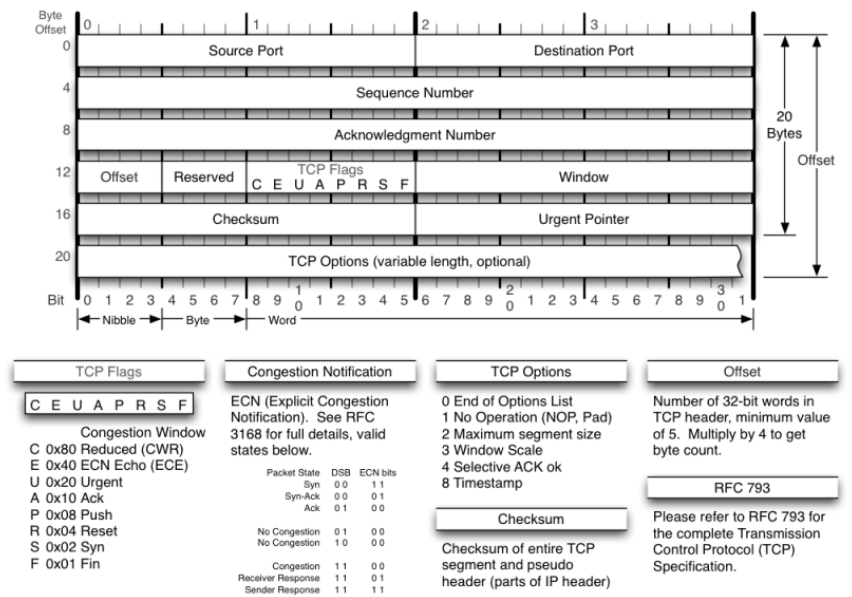
\includegraphics[width=0.8\linewidth]{img/tcp}
\end{figure}

\paragraph{Three-way Handshake}
\begin{enumerate}
\item Client sends \texttt{SYN} with its ISN.
\item Server responds with both:
\begin{enumerate}
\item \texttt{SYN} with its ISN.
\item \texttt{ACK} with the first unseen client sequence number.
\end{enumerate}
\item Client responds with \texttt{ACK} with the first unseen server sequence
number, and its new sequence number.
\end{enumerate}
\emph{Disconnection} uses \texttt{FIN} instead of \texttt{SYN}, and
usually two exchanges.
\begin{figure}[H]
\centering{}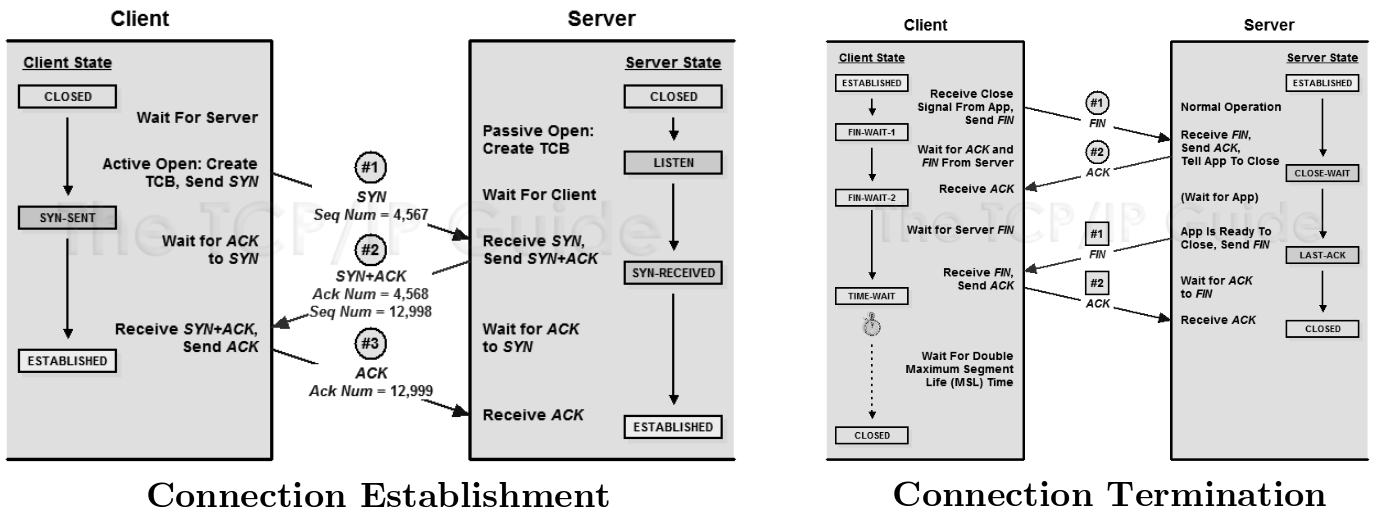
\includegraphics[width=1\linewidth]{img/handshake}
\end{figure}

\paragraph{States}

Use \texttt{netstat -at} to see current TCP connection states.
\begin{figure}[H]
\centering{}%
\begin{minipage}[t]{0.5\columnwidth}%
Client:
\begin{center}
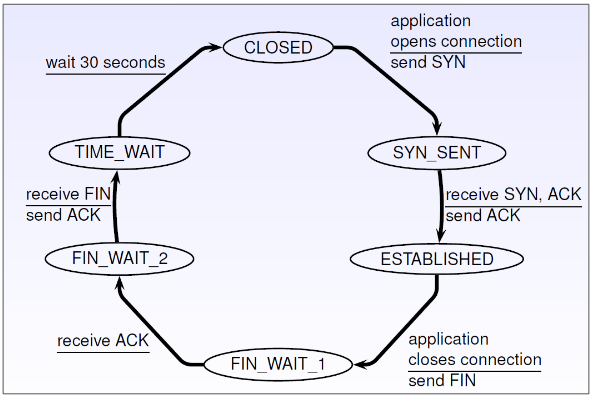
\includegraphics[width=0.8\linewidth]{img/client-states}
\par\end{center}%
\end{minipage}%
\begin{minipage}[t]{0.5\columnwidth}%
Server:
\begin{center}
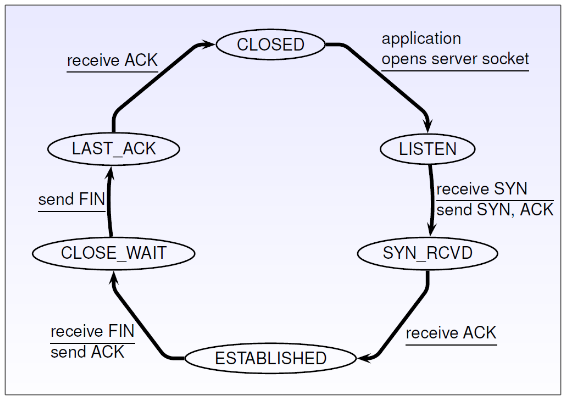
\includegraphics[width=0.8\linewidth]{img/server-states}
\par\end{center}%
\end{minipage}
\end{figure}

\subsection{Error Detection and Retransmission}
\begin{itemize}
\item TCP adds reliability on top of unreliable data-link layer. Bit errors
can occur, hence we use a checksum.
\item \emph{Error detection}: use a checksum.
\item \emph{Receiver feedback}: if packet is corrupted, wrong or timeout:
\begin{itemize}
\item Could send a \texttt{NACK}, protected with an error-detection code.
\begin{itemize}
\item Corrupted \texttt{ACK}s are interpreted as \texttt{NACK}s.
\item We may get \emph{duplicate} segments, which we can ignore using SEQ
numbers.
\begin{itemize}
\item SEQ number may be a single bit (\emph{alternating bit protocol}).
\end{itemize}
\end{itemize}
\item Could send an \texttt{ACK} for the next needed byte. Many methods:
\begin{itemize}
\item \emph{Delayed}: wait for the next segment, if it doesn't arrive, send
\texttt{ACK}.
\item \emph{Cumulative}: send \texttt{ACK} for multiple segments at once.
\item \emph{Duplicate}: send another \texttt{ACK} if an out of order segment
arrives.
\item \emph{Immediate}: immediately send an \texttt{ACK} for the first gap.
\end{itemize}
\end{itemize}
\end{itemize}

\paragraph{Congestion Control}

Aims not to overflow the network.
\begin{itemize}
\item \emph{Congestion window}: how many bytes can be pushed before waiting
for an acknowledgement. I.e. last byte sent - last byte \texttt{ACK}ed
$\leq W$.
\begin{itemize}
\item Where $W=\min\left(\text{congestion window},\text{receiver window}\right)$.
\item The resulting maximum output rate $\lambda=\frac{W}{RTT}$.
\end{itemize}
\item \emph{Slow Start}:
\begin{itemize}
\item Initial $W$ is $MSS$.
\item Double $W$ every $RTT$, until:
\begin{itemize}
\item $W>$ sshthresh, then use Congestion Avoidance.
\item $W=$ sshthresh, then use either Slow Start or Congestion Avoidance.
\end{itemize}
\end{itemize}
\item \emph{Congestion Avoidance}:
\begin{itemize}
\item $W=W+MSS\times\frac{MSS}{W}$ ($W$ increased by approximately 1 $MSS$
every $RTT$).
\end{itemize}
\item \emph{AIMD Additive-Increase / Multiplicative-Decrease}:
\begin{itemize}
\item $W$ is increased with every good acknowledgement by CA.
\item $W$ is halved at every packet loss event.
\end{itemize}
\item \emph{Reliability and Timeout}:
\begin{itemize}
\item Timeout should be longer than $RTT$ (to avoid unnecessary retransmissions)
but not too long (to detect and retransmit lost segments quickly).
\item Use $T=\overline{RTT}+4\times\overline{DevRTT}$, based on estimated
$RTT$ (get by ping).
\end{itemize}
\item \emph{Fast Recovery}: three duplicate \texttt{ACK}s interpreted as
a \texttt{NACK}.
\begin{itemize}
\item Timeout:
\begin{itemize}
\item Set sshthresh to half the current window size.
\item Go back to $W=MSS$ and run SS.
\end{itemize}
\item \texttt{NACK}: Cut $W$ in half and run CA.
\end{itemize}
\end{itemize}

\paragraph{Flow Control}

Aims not to overflow the receiver.
\begin{itemize}
\item Receiver sends its window size (max number of bytes that can be sent)
along with its acknowledgement.
\item A window size of 0 is valid.
\end{itemize}

\paragraph{Wireless TCP}

TCP assumes IP is running over wires. When packets are lost, TCP assumes
congestion and slows down. Possible solutions:
\begin{enumerate}
\item Split TCP to distinguish between wired and wireless IP.
\item Let the base station do some transmissions without informing the source.
\end{enumerate}

\subsection{UDP}
\begin{itemize}
\item No flow control, error control, retransmissions.
\item Datagrams cannot be larger than 65K. (Usually use 500B or less).
\end{itemize}
Useful for:
\begin{itemize}
\item Finer Application Level control over what data are sent and when (e.g.
real-time: Skype).
\item No connection establishment (faster).
\item Non connection state.
\item Small packet header overhead.
\end{itemize}

\subsubsection*{Header Fields}

\begin{figure}[H]
\centering{}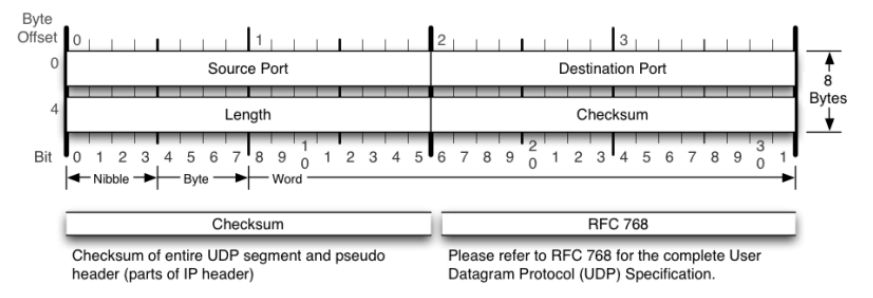
\includegraphics[width=0.75\linewidth]{img/udp}
\end{figure}

\subsection{Network Usage}

\[
\text{Utilisation Factor}=\frac{\text{how much we actually used the network}}{\text{how much we could have used it}}
\]

\section{Network Security}

\subsection{Terminology}
\begin{itemize}
\item \emph{Hacker}: once skilled, now cybercriminals. White/black/grey
hats.
\item \emph{Virii}: e.g. ransomware/spyware/Trojans.
\item \emph{Anarchists}: physical.
\item \emph{Crackers}: use others' tools to infiltrate systems.
\item \emph{DDoSers}: participants in distributed denial of service attacks.
\item \emph{Spammers/botters}: mass senders of spam messages.
\item \emph{Pirates}: upload or download illegal content.
\item \emph{Cyberbullies}: harass, stalk, offend, threaten users.
\item \emph{Whistleblowers}: reveal inside secrets.
\item \emph{Social engineers/phishers/catfishes}: manipulators, pretend
to be somebody else.
\end{itemize}

\paragraph{Black Hat Tools}
\begin{itemize}
\item \emph{Rootkits}: allow attackers to enter system.
\item \emph{Keyloggers}.
\item \emph{Trojans}: allow remote control of a system.
\item \emph{Evil twin}: free WiFi networks, sniff everything you send.
\end{itemize}

\paragraph{White Hat Tools}
\begin{itemize}
\item \emph{Tails}: OS that forgets everything.
\item \emph{Kali Linux}: provides security and pentesting tools.
\item \emph{Metasploit}: like \texttt{nmap}, identifies systems and vulns.
\end{itemize}

\paragraph{Network Security Issues}
\begin{itemize}
\item \emph{Access control}: only certain users are allowed to access a
resource.
\item \emph{Authentication}: user knows that the resource really is what
it says it is, and v.v.
\item \emph{Confidentiality}: user limits access to information / resources
they own. (Encryption).
\item \emph{Integrity}: actions of a user should not affect integrity of
resource.
\item \emph{Non-repudiation}: users cannot deny communication took place.
(Monitoring, logging, auditing).
\end{itemize}

\subsection{Firewalls}

\paragraph{Access Control}

In a \emph{secure channel}, the \emph{guard} (e.g. firewall) controls:
\begin{itemize}
\item Which principals can access the resource.
\item Where principals are allowed to be located.
\item What requests principals are allowed to make.
\end{itemize}
A firewall:
\begin{itemize}
\item Controls access to the network (gateway between \emph{internal} and
\emph{external} networks).
\item Analyses inbound packets, and blocks / allows based on rules.
\end{itemize}
Examples:
\begin{itemize}
\item \emph{Application-level gateway}: runs on the host.
\begin{itemize}
\item Can block based on application-level content.
\end{itemize}
\item \emph{Proxy server}: runs on the entire network, can protect entire
LAN.
\begin{itemize}
\item Private network only accessible via proxy.
\end{itemize}
\item \emph{Circuit-level gateway}: act like a non-caching proxy.
\item \emph{Packet filtering}:
\begin{itemize}
\item \emph{Stateless}: checks source / destination IP address and ports.
\item \emph{Stateful}: remembers connections and check contents of current
and previous packets.
\end{itemize}
\end{itemize}

\paragraph{Bastion Hosts}

External hosts which expect to be attacked.
\begin{itemize}
\item Performs auditing / logging.
\item Runs a trusted and secure OS.
\item Administered via dedicated terminal.
\item Only run necessary software, set file permissions, turn on quotas,
process limits, remove regular user accounts, make filesystem read
only, ....
\end{itemize}
Responsibilities:
\begin{itemize}
\item Relays connections and maintains state.
\item Can authenticate users.
\item Can drop connections if necessary.
\end{itemize}

\paragraph{Demilitarized Zone}

Area between you and the outside.
\begin{itemize}
\item External hosts can only speak directly to your internal hosts within
the DMZ.
\item All other non-DMZ hosts are protected by the gateway/router/firewall.
\item Router uses NAT (network address translation) to get external messages
to correct internal host.
\item If you want to expose an internal host without putting it in the DMZ,
you must \emph{port forward} (from a given port of router's public
IP to a given port of host's NAT-based LAN IP).
\end{itemize}

\paragraph{Getting Around Firewalls}
\begin{itemize}
\item \texttt{ssh}.
\item Spoof MAC/IP.
\item Use a VPN (virtual private network) to tunnel around a firewall.
\begin{itemize}
\item Firewall won't be able to know what you're doing.
\item As long as your tunnel uses SSL (secure sockets layer) / TLS (transport
security layer).
\end{itemize}
\end{itemize}

\paragraph{Access Control Lists}

Packet filtering rules.
\begin{itemize}
\item Rules are checked top to bottom. Allow what you need, block everything
else or v.v.
\item E.g. use \texttt{iptables} and \texttt{tcpd} to edit access control
lists.
\end{itemize}

\paragraph{Keywords}
\begin{itemize}
\item \emph{IDS}: intrusion detection system.
\item \emph{IPS}: intrusion protection system.
\item \emph{NGFW}: next generation firewall: stateful firewall with IPS/IDS.
\item \emph{UMT}: unified thread management: NGFW but with extra capabilities
(e.g. antispam/antivirus).
\end{itemize}

\subsection{Cryptography}

\begin{figure}[H]
\centering{}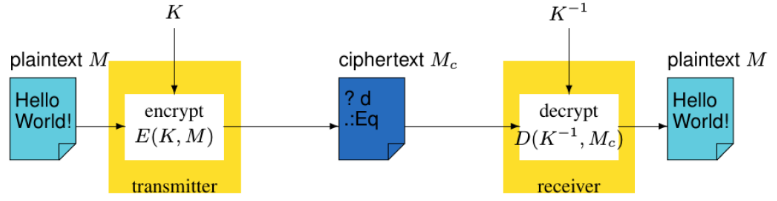
\includegraphics[width=0.75\linewidth]{img/encryption}
\end{figure}

\paragraph{Symmetric (Secret Key) Encryption}
\begin{itemize}
\item $K=K^{-1}$.
\item $K$ must be carefully distributed.
\end{itemize}

\paragraph{Asymmetric (Public Key) Encryption}
\begin{itemize}
\item $K$ is the \emph{private-key}.
\item $K^{-1}$ is the \emph{public-key}.
\item Successfully decrypting the message using public key \emph{authenticates}
that the message came from the correct transmitter.
\item Encrypting a message with the receiver's public key ensures \emph{confidentiality}
since only they can decrypt it.
\item More secure but slower than symmetric encryption.
\end{itemize}

\paragraph{Secure Channel Establishment}
\begin{enumerate}
\item Agree on a new key. \emph{Diffie-Hellman} key exchange:
\begin{enumerate}
\item Choose a generator $g$ and large prime $p$.
\item Bob chooses a secret $b$ and Alice a secret $a$.
\item Bob calculates $x=g^{b}\mod p$ and Alice $y=g^{a}\mod p$, and share
these.
\item They then calculate $y^{b}\mod p=\left(g^{a}\mod p\right)^{b}$ and
$x^{a}\mod p=\left(g^{b}\mod p\right)^{a}$ respectively. The final
key is $g^{ab}\mod p$.
\end{enumerate}
\item Use trusted secure hosts. Obtain a key from the trusted host securely.
\end{enumerate}

\section{Network Layer}

Provides facilities for getting data from a source to a destination.
\begin{itemize}
\item May make many hops (\emph{routing}).
\item Must know network \emph{topology} to choose appropriate paths.
\item Requires \emph{load balancing} along routes.
\item Has to deal with \emph{network heterogeneity}.
\end{itemize}

\paragraph{Router}
\begin{itemize}
\item Has \emph{interfaces} (physical ports).
\end{itemize}

\paragraph{Forwarding}
\begin{itemize}
\item Potentially multiple, asymmetric paths.
\item Routers cooperate to find the best routes, by building a \emph{sink
tree} with \emph{optimal routes}.
\item Use \texttt{traceroute} command to see.
\end{itemize}

\paragraph{Routing Algorithms}
\begin{itemize}
\item \emph{Shortest path routing}: calculate using Dijkstra's algorithm.
\item \emph{Flood routing}: forward incoming packet across every outgoing
link.
\begin{itemize}
\item Always chooses \emph{shortest path}.
\item Increases \emph{overhead}.
\item Makes sense when \emph{robustness} is required.
\end{itemize}
\begin{enumerate}
\item After a packet was forwarded across $N$ routers (\emph{hop counter}
$>N$), discard it.
\item Avoid directed cycles by forwarding only once.
\item Flood selectively, only in direction that makes sense.
\end{enumerate}
\item \emph{Distance vector routing}: dynamic protocol that uses Bellman-Ford:
\begin{itemize}
\item Good news propagates quickly.
\item Bad news propagates slowly (count-to-infinity problem). Use a longest
acceptable path to avoid this.
\end{itemize}
\begin{enumerate}
\item Consider costs that direct neighbours advertise to get packet to destination.
\item Select neighbour whose advertised cost + cost to get to that neighbour
is lowest.
\item Advertise new cost to neighbours.
\end{enumerate}
\item \emph{Link state routing}:
\begin{enumerate}
\item Discover direct neighbours and get their addresses.
\item Calculate cost for sending packet to each neighbour.
\item Construct LSA (link state advertisement) packet with all information.
\item Send / collect packet to / from \emph{all} other routers.
\item Run Dijkstra's algorithm locally to find shortest paths.
\end{enumerate}
\end{itemize}
\begin{table}[H]
\centering{}%
\begin{tabular}{ccc}
\toprule 
 & \textbf{DVR} & \textbf{LSR}\tabularnewline
\midrule
Network knowledge & Local & Global\tabularnewline
Computation & Global & Local\tabularnewline
Synchronisation & Gradual & ``Instant''\tabularnewline
\bottomrule
\end{tabular}
\end{table}
\begin{itemize}
\item \emph{Hierarchical routing}: routing algorithm that can scale!
\begin{itemize}
\item Go for suboptimal routes by introducing \emph{regions}, and separate
algorithms for intra-region and inter-region routing.
\end{itemize}
\item \emph{Broadcast routing}: attempt to send message to every host on
network:
\begin{itemize}
\item Use \emph{flood routing}, if we can \emph{limit} flood.
\item Multi-destination routing approach, requires list of all destinations.
\item \emph{Multicast}. Build a sink tree and use for multicast route.
\end{itemize}
\item \emph{Multicast routing}:
\begin{itemize}
\item \emph{Solution 1}: Construct a spanning tree at each router using
RPF (reverse-path forwarding).
\begin{itemize}
\item Each router broadcasts packet to every adjacent router, except where
it came from.
\item Accept packet only if it arrives on a direct path from origin.
\end{itemize}
\item Use a group ID to prune paths to nodes that do not contain members
of the group.
\item \emph{Solution 2}: Use \emph{core-based trees}.
\begin{itemize}
\item Single spanning tree per group with root near middle.
\item Hosts send multicasts to core.
\item Not optimal for all sources, but more scaleable.
\end{itemize}
\end{itemize}
\end{itemize}

\paragraph{Internetworking}

Construct gateways that interconnect different kinds of networks.
\begin{itemize}
\item \emph{PAN}: personal area network, e.g. hotspot between phone and
laptop.
\item \emph{LAN}: local area network, multiple users for the same purpose.
\item \emph{MAN}: metropolitan area network.
\item \emph{WAN}: wide area network, e.g. the Internet.
\end{itemize}

\paragraph{Devices}
\begin{itemize}
\item \emph{Repeaters} / \emph{hubs}: physical layer devices that boost
signals.
\item \emph{Switches}, \emph{bridges}: data link layer devices that make
\emph{interconnections} based on MAC address.
\item Multi-protocol \emph{routers} / \emph{gateways}: network layer devices
that make decisions based on IP address.
\end{itemize}

\paragraph{The Internet}

Collection of \emph{autonomous systems} connected by \emph{backbones}.
\begin{itemize}
\item \emph{Gateway routers} interconnect autonomous systems.
\item Use \emph{hierarchical routing}:
\begin{itemize}
\item \emph{Intra-AS routing protocols}: RIP (distance vector) and open
shortest path first OSPF (link state).
\item \emph{Inter-AS routing protocols}: BGP.
\end{itemize}
\end{itemize}

\paragraph{Border Gateway Protocol}
\begin{itemize}
\item Neighbouring routers maintain connection to simplify reliability:
provides reachability information from neighbour ASs.
\item Determines routes to all outside subnets based on reachability information
and policies.
\item Path-vector protocol, based on distance-vector routing but paths instead
of distances announced.
\item Routers advertise routes to networks.
\begin{itemize}
\item Destinations denoted by address prefixes.
\item May aggregate prefixes (\emph{supernetting}).
\end{itemize}
\item \emph{Autonomous system number} (ASN): uniquely identifies each AS.
\item BGP attributes: include AS-PATH and NEXT-HOP.
\item BGP import policy: decides whether to accept or reject route advertisement.
\end{itemize}

\subsection{Internet Protocol}

\emph{Best-effort}: a packet-switched connectionless service.
\begin{itemize}
\item Datagram format.
\item Fragmentation.
\item Addressing.
\item Packet handling.
\end{itemize}

\paragraph{Fragmentation}
\begin{itemize}
\item If input datagram exceeds MTU of output link, IP datagram must be
\emph{fragmented}.
\item Destination reassembles fragmented datagrams.
\item \emph{Fragment offset} is offset in units of 8 bytes.
\item \emph{Total length} is the number of bits in this fragment.
\item \emph{More fragments} flag will be set if more fragments are expected
to follow.
\end{itemize}
\begin{figure}[H]
\centering{}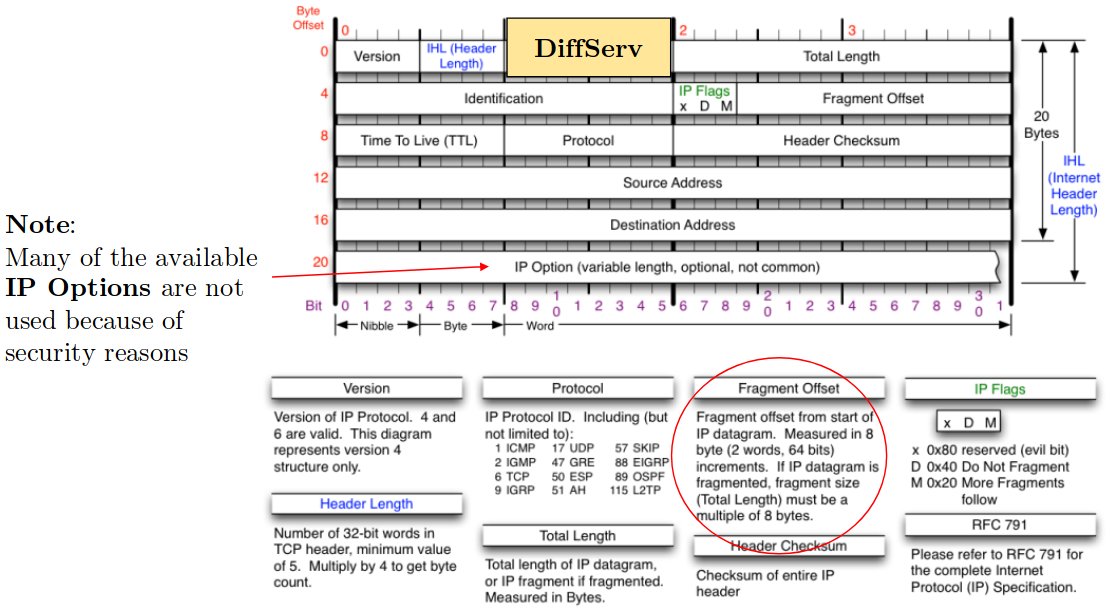
\includegraphics[width=0.95\linewidth]{img/ip}
\end{figure}

\subsubsection{IPv4 Addressing}

Each IP address is a associated with an interface.

\paragraph{Classful Addressing}

No longer used:
\begin{itemize}
\item Class A: 0NNNNNNN.HHHHHHHH.HHHHHHHH.HHHHHHHH.
\item Class B: 10NNNNNN.NNNNNNNN.HHHHHHHH.HHHHHHHH.
\item Class C: 110NNNNN.NNNNNNNN.NNNNNNNN.HHHHHHHH.
\item Class D: 1110....: multicast address.
\item Class E: 1111....: reserved for future use.
\end{itemize}

\paragraph{Subnet Masking}

Use a single network address for entire organisation, and divide internally
into subnet addresses and host ids.
\begin{itemize}
\item \emph{Classless Inter-Domain Routing} (CIDR) notation: address/prefix-length.
\item Subnet mask for length $p$ is $p$ 1's followed by $32-p$ 0's.
\item Network name is given first IP.
\item First IP of a host is the router.
\item Last IP is the broadcast address.
\end{itemize}

\paragraph{Longest Prefix Matching}

Choose entry that matches destination address with longest prefix.
\begin{itemize}
\item 0.0.0.0/0 is the \emph{default route} (otherwise broadcast).
\end{itemize}

\paragraph{Network Address Translation}

Assign each company / home a single IP, each device gets a unique
local IP.
\begin{itemize}
\item Several private address ranges exist for local networks.
\item You can find out your local IP, you can use \texttt{ifconfig}.
\item When a connection is set up from a local IP on port X, the router
uses its public address on port Y, and registers a mapping.
\item Incoming connections require a static mapping from a port on the public
address to a given port on a local address.
\end{itemize}
Criticism:
\begin{enumerate}
\item Violates architectural IP model of IP address uniquely identifying
a machine.
\item Makes internet a connection-oriented network.
\item NAT makes assumptions about TCP, cannot easily support new transport
protocols.
\item Uses behind NAT cannot be contact directly without port forwarding.
\end{enumerate}
IPv6 could help deal with lack of IP addresses.

\subsubsection{IPv6 Addressing}
\begin{itemize}
\item Expanded addressing, supports anycast.
\item Fragmentation done at end systems.
\item Remove header checksum, since the transport protocols do this already.
\item Remove options.
\end{itemize}

\subsection{Internet Control Message Protocol}
\begin{itemize}
\item Error reporting.
\item Signalling.
\end{itemize}
E.g. used for \texttt{ping}.

\subsection{Dynamic Host Configuration Protocol}

Address configuration.
\begin{itemize}
\item Each new machine broadcasts DHCP DISCOVER packet when it connects.
\item DHCP server replies with the assigned IP address.
\item Mapping may be static, or assign different addresses each time a host
connects.
\end{itemize}

\section{Data Link Layer}

\subsection{Ethernet}

\paragraph{Cables}

Goal is to protect against electromagnetic interference (EMI):
\begin{itemize}
\item \emph{UTP} (unshielded twisted pair).
\item STP (shielded/screened twisted pair).
\item \emph{FTP} (foiled twisted pair).
\item \emph{SFTP} (shielded and foiled twisted pair).
\end{itemize}

\paragraph{Pinouts}
\begin{itemize}
\item \emph{Straight-through}: communicate between \emph{different} OSI
layers.
\item \emph{Crossover} (media dependent interface MDI): communicate between
devices of the \emph{same} OSI layer.
\item \emph{Rollover} (media dependent interface with crossover MDIX): directly
tap into a networking device.
\end{itemize}

\paragraph{Switches}
\begin{itemize}
\item Forwards messages out of the right port.
\item Uses a forwarding information base (FIB) MAC table.
\end{itemize}

\paragraph{Frames}
\begin{itemize}
\item Has a cyclic redundancy check (CRC) checksum in the footer).
\end{itemize}
\begin{figure}[H]
\centering{}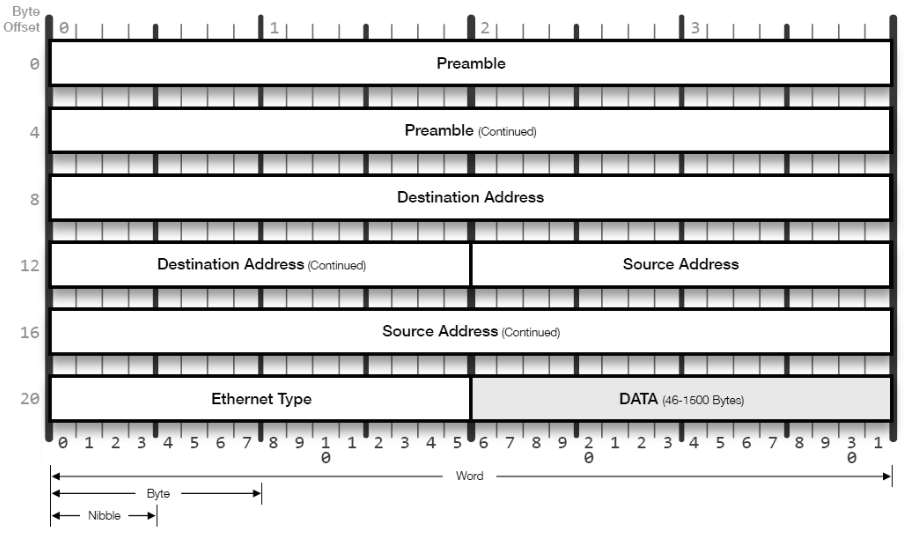
\includegraphics[width=0.75\linewidth]{img/ethernet}
\end{figure}

\paragraph{MAC Addressing}
\begin{itemize}
\item Each network interface card (NIC) has a MAC address.
\item 48 bits / 6 bytes.
\item 8th (I/G) bit decides if individual or group address.
\item 7th (U/L) bit decides if universally or locally administered.
\item FF:FF:FF:FF:FF:FF is the \emph{broadcast address}.
\item IP is linked to MAC address, so routers can explain to switches which
host a packet is for.
\end{itemize}

\paragraph{Address Resolution Protocol}

Use \texttt{arp} to see what your computer knows. Use \texttt{tcpdump}
to see communication.
\begin{enumerate}
\item \emph{Router}: asks each host on LAN if they have the request IP.
(Broadcasts a frame).
\begin{itemize}
\item \texttt{arp who has host\_ip tell router\_ip (router\_mac)}
\end{itemize}
\item \emph{Host}: checks it has the requested address, if so, send reply
with its MAC.
\begin{itemize}
\item \texttt{arp reply host\_ip is\_at host\_mac (router\_mac)}
\end{itemize}
\item \emph{Router}: receive ARP message and caches IP and MAC.
\end{enumerate}

\subsection{Network Topologies}

\begin{figure}[H]
\centering{}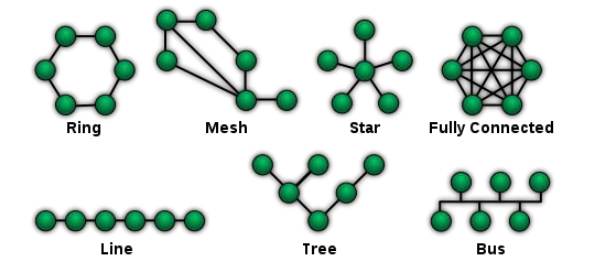
\includegraphics[width=0.5\linewidth]{img/network-topologies}
\end{figure}
\begin{itemize}
\item \emph{Bus}: used main coaxial cable to connect all hosts, use a BNC
coaxial T connectors and terminators. 
\item \emph{Ring}: requires 2 NICs per host. If a link gets cut, network
dies. Also \emph{dual-ring} which requires 4 NICs per host.
\begin{itemize}
\item \emph{Fibre Distributed Data Interface} (FDDI): supports long distance
transmission, and can short circuit two rings together.
\end{itemize}
\item \emph{Token ring}: connect all hosts to a multi-station access unit
(MSAU). Data flows by passing around a token.
\begin{itemize}
\item \emph{Frames}: \emph{access control} bit at the start of all frames
to identify presence of token, \emph{frame status} bit to say whether
address was found, \emph{inter-frame gaps} to separate them.
\item \emph{Active monitor}: takes responsibility for generating tokens,
any host must be able to do this.
\item \emph{Concentrators} avoid single failures breaking links by switching
out faulty hosts.
\end{itemize}
\item \emph{Star}: no token. Central device is a single point of failure
(SPoF).
\item \emph{Line}: ring that doesn't meet at the ends (terrible).
\item \emph{Tree}: a star bus.
\item \emph{Mesh}: some connected to some. More fault tolerant, but expensive.
\item \emph{Fully connected}: expensive and difficult to manage.
\item \emph{Hybrid}: mix of topologies.
\end{itemize}

\subsection{Medium Access Control}

Coordinates channel access.
\begin{itemize}
\item A separate layer within the Data Link layer (the other is Logical
Link Control). 
\end{itemize}

\paragraph{Strategies}
\begin{enumerate}
\item \emph{No control}. let stations retransmit after collision.
\begin{itemize}
\item Fine if utilisation is low, otherwise very inefficient.
\end{itemize}
\item \emph{Round-robin}. stations take turns using the channel.
\begin{itemize}
\item Used by \emph{token-based} MAC systems - only station with the token
can transmit.
\end{itemize}
\item \emph{Reservation}: stations obtain channel reservation before transmitting.
\begin{itemize}
\item Used in \emph{slotted} systems - need to manage reservations.
\end{itemize}
\end{enumerate}

\paragraph{Static Channel Allocation}
\begin{enumerate}
\item \emph{Time division multiplexing} (TDM): station must wait its turn
to transmit.
\item \emph{Frequency division multiplexing} (FDM): station must use only
limited frequency band.
\end{enumerate}

\paragraph{Dynamic Channel Allocation}
\begin{enumerate}
\item \emph{ALOHA}: When a station has a frame to be transmitted, send it.
When collisions occur, wait a \emph{random} amount of time and retry.
\item \emph{Slotted ALOHA}: Only specific time slots when stations may transmit.
\begin{enumerate}
\item \emph{Carrier sensing}: transmission only allowed when channel is
idle.
\begin{enumerate}
\item \emph{CSMA/CD}: Carrier sense multiple access / collision detection
(Ethernet).
\item \emph{CSMA/CA}: Carrier sense multiple access / collision avoidance
(WiFi).
\end{enumerate}
\end{enumerate}
\end{enumerate}

\paragraph{Collision Detection}
\begin{itemize}
\item Station senses channel while transmitting to know whether its frame
is OK.
\item \emph{CD}: transmission stops after collision, add \emph{jamming signal}.
\item Host must transmit for long enough to know frame is OK (min length
is $2n$ where $n$ is end-to-end transmission delay).
\end{itemize}

\paragraph{Back-Off}
\begin{itemize}
\item \emph{1-persistant CSMA}: Station keeps checking if the channel is
free and then transmits immediately.
\item \emph{Non-persistent CSMA}: If channel is busy, wait for a random
amount of time before checking again and then transmit immediately.
\item \emph{$p$-persistent CSMA}: Station keeps checking if channel is
free and transmits with probability $p$.
\item \emph{Binary exponential back-off}: after $c$ collisions, choose
slot in range $0$ to $2^{c}-1$ for next attempt. Give up after 10
collisions (1023 upper limit).
\end{itemize}

\paragraph{Token Passing}

An alternative to CSMA/CD.
\begin{itemize}
\item Collisions are inevitable using CSMA/CD, stations may be delayed indefinitely.
\end{itemize}

\paragraph{Carrier Extension}

Pad any packet up to 512 bytes.

\paragraph{Frame Bursting}

Allow host to send multiple frames: many short frames with carrier
in between.

\paragraph{Switched topology}

One host on each port to avoid collisions. Switches only transmit
when channel available.

\section{Physical Layer}

\subsubsection*{Cables}

\begin{table}[H]
\centering{}%
\begin{tabular}{cc}
\toprule 
 & \textbf{Repeater Spacing}\tabularnewline
\midrule
\emph{Twisted Pair} & 2km\tabularnewline
\emph{Coaxial Cable} & 1-9km\tabularnewline
\emph{Fibre Optic} & 40km\tabularnewline
\bottomrule
\end{tabular}
\end{table}
\begin{itemize}
\item Attenuation, bandwidth.
\end{itemize}

\paragraph{Patch Panels}

Connects sockets to switches.

\paragraph{Wireless Transmission}
\begin{itemize}
\item Convenient when communication required without wires.
\item Bidirectional by default.
\end{itemize}

\paragraph{Information Representation}
\begin{itemize}
\item \emph{Baud rate}: symbol rate per second.
\item \emph{Bitrate}: how many times per unit \emph{can} the symbol change?
\end{itemize}
%
\begin{itemize}
\item A digital channel can be implemented by an analogue channel using
a \emph{modem}.
\item An analogue channel can be implemented by a digital channel using
a \emph{codec}.
\end{itemize}

\paragraph{Properties of Signals}

\[
c=f\lambda
\]

If $\lambda$ is in meters and $f$ is in MHz, $\lambda f\approx300$.
\begin{itemize}
\item \emph{Waveform}: shape.
\item \emph{Amplitude}: range.
\item \emph{Wavelength}: distance signal travels before repetition.
\item \emph{Frequency}: number of repetitions per unit time.
\end{itemize}

\paragraph{Modulation}

Encode digital information signal to be transmitted effectively using
bandwidth supported by a channel.
\begin{itemize}
\item \emph{Baseband modulation}: unmodified.
\item \emph{Broadband modulation}: use physical carrier signal to encode
information signal.
\begin{itemize}
\item \emph{Amplitude modulation} (ASK): carrier frequency is modulated
in amplitude (prone to interference).
\item \emph{Frequency modulation} (PSK).
\item \emph{Phase modulation} (PSK): phase change represents a 1 bit.
\item More advanced modulation techniques transmit multiple bits per symbol
- using combination of modulation schemes.
\end{itemize}
\end{itemize}

\paragraph{DSL}
\begin{itemize}
\item Conventional phone lines can only reach 56Kbps download speed, limited
to 3000Hz bandwidth.
\item DSL (digital subscriber line) removes the bandwidth filter.
\item ADSL (asymmetric). E.g. divides 1.1MHz bandwidth into 256 channels
of 4000Hz each, mostly allocated to download.
\end{itemize}

\end{document}
